\documentclass[1p]{elsarticle_modified}
%\bibliographystyle{elsarticle-num}

%\usepackage[colorlinks]{hyperref}
%\usepackage{abbrmath_seonhwa} %\Abb, \Ascr, \Acal ,\Abf, \Afrak
\usepackage{amsfonts}
\usepackage{amssymb}
\usepackage{amsmath}
\usepackage{amsthm}
\usepackage{scalefnt}
\usepackage{amsbsy}
\usepackage{kotex}
\usepackage{caption}
\usepackage{subfig}
\usepackage{color}
\usepackage{graphicx}
\usepackage{xcolor} %% white, black, red, green, blue, cyan, magenta, yellow
\usepackage{float}
\usepackage{setspace}
\usepackage{hyperref}

\usepackage{tikz}
\usetikzlibrary{arrows}

\usepackage{multirow}
\usepackage{array} % fixed length table
\usepackage{hhline}

%%%%%%%%%%%%%%%%%%%%%
\makeatletter
\renewcommand*\env@matrix[1][\arraystretch]{%
	\edef\arraystretch{#1}%
	\hskip -\arraycolsep
	\let\@ifnextchar\new@ifnextchar
	\array{*\c@MaxMatrixCols c}}
\makeatother %https://tex.stackexchange.com/questions/14071/how-can-i-increase-the-line-spacing-in-a-matrix
%%%%%%%%%%%%%%%

\usepackage[normalem]{ulem}

\newcommand{\msout}[1]{\ifmmode\text{\sout{\ensuremath{#1}}}\else\sout{#1}\fi}
%SOURCE: \msout is \stkout macro in https://tex.stackexchange.com/questions/20609/strikeout-in-math-mode

\newcommand{\cancel}[1]{
	\ifmmode
	{\color{red}\msout{#1}}
	\else
	{\color{red}\sout{#1}}
	\fi
}

\newcommand{\add}[1]{
	{\color{blue}\uwave{#1}}
}

\newcommand{\replace}[2]{
	\ifmmode
	{\color{red}\msout{#1}}{\color{blue}\uwave{#2}}
	\else
	{\color{red}\sout{#1}}{\color{blue}\uwave{#2}}
	\fi
}

\newcommand{\Sol}{\mathcal{S}} %segment
\newcommand{\D}{D} %diagram
\newcommand{\A}{\mathcal{A}} %arc


%%%%%%%%%%%%%%%%%%%%%%%%%%%%%5 test

\def\sl{\operatorname{\textup{SL}}(2,\Cbb)}
\def\psl{\operatorname{\textup{PSL}}(2,\Cbb)}
\def\quan{\mkern 1mu \triangleright \mkern 1mu}

\theoremstyle{definition}
\newtheorem{thm}{Theorem}[section]
\newtheorem{prop}[thm]{Proposition}
\newtheorem{lem}[thm]{Lemma}
\newtheorem{ques}[thm]{Question}
\newtheorem{cor}[thm]{Corollary}
\newtheorem{defn}[thm]{Definition}
\newtheorem{exam}[thm]{Example}
\newtheorem{rmk}[thm]{Remark}
\newtheorem{alg}[thm]{Algorithm}

\newcommand{\I}{\sqrt{-1}}
\begin{document}

%\begin{frontmatter}
%
%\title{Boundary parabolic representations of knots up to 8 crossings}
%
%%% Group authors per affiliation:
%\author{Yunhi Cho} 
%\address{Department of Mathematics, University of Seoul, Seoul, Korea}
%\ead{yhcho@uos.ac.kr}
%
%
%\author{Seonhwa Kim} %\fnref{s_kim}}
%\address{Center for Geometry and Physics, Institute for Basic Science, Pohang, 37673, Korea}
%\ead{ryeona17@ibs.re.kr}
%
%\author{Hyuk Kim}
%\address{Department of Mathematical Sciences, Seoul National University, Seoul 08826, Korea}
%\ead{hyukkim@snu.ac.kr}
%
%\author{Seokbeom Yoon}
%\address{Department of Mathematical Sciences, Seoul National University, Seoul, 08826,  Korea}
%\ead{sbyoon15@snu.ac.kr}
%
%\begin{abstract}
%We find all boundary parabolic representation of knots up to 8 crossings.
%
%\end{abstract}
%\begin{keyword}
%    \MSC[2010] 57M25 
%\end{keyword}
%
%\end{frontmatter}

%\linenumbers
%\tableofcontents
%
\newcommand\colored[1]{\textcolor{white}{\rule[-0.35ex]{0.8em}{1.4ex}}\kern-0.8em\color{red} #1}%
%\newcommand\colored[1]{\textcolor{white}{ #1}\kern-2.17ex	\textcolor{white}{ #1}\kern-1.81ex	\textcolor{white}{ #1}\kern-2.15ex\color{red}#1	}

{\Large $\underline{12a_{1006}~(K12a_{1006})}$}

\setlength{\tabcolsep}{10pt}
\renewcommand{\arraystretch}{1.6}
\vspace{1cm}\begin{tabular}{m{100pt}>{\centering\arraybackslash}m{274pt}}
\multirow{5}{120pt}{
	\centering
	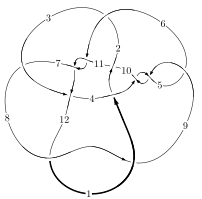
\includegraphics[width=112pt]{../../../GIT/diagram.site/Diagrams/png/1807_12a_1006.png}\\
\ \ \ A knot diagram\footnotemark}&
\allowdisplaybreaks
\textbf{Linearized knot diagam} \\
\cline{2-2}
 &
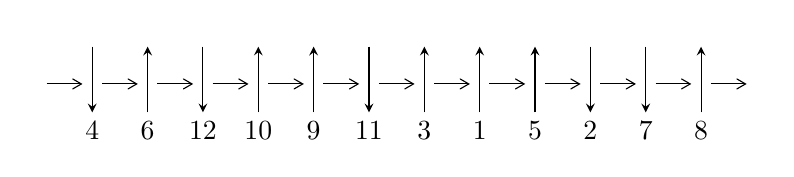
\begin{tikzpicture}[x=20pt, y=17pt]
	% nodes
	\node (C0) at (0, 0) {};
	\node (C1) at (1, 0) {};
	\node (C1U) at (1, +1) {};
	\node (C1D) at (1, -1) {4};

	\node (C2) at (2, 0) {};
	\node (C2U) at (2, +1) {};
	\node (C2D) at (2, -1) {6};

	\node (C3) at (3, 0) {};
	\node (C3U) at (3, +1) {};
	\node (C3D) at (3, -1) {12};

	\node (C4) at (4, 0) {};
	\node (C4U) at (4, +1) {};
	\node (C4D) at (4, -1) {10};

	\node (C5) at (5, 0) {};
	\node (C5U) at (5, +1) {};
	\node (C5D) at (5, -1) {9};

	\node (C6) at (6, 0) {};
	\node (C6U) at (6, +1) {};
	\node (C6D) at (6, -1) {11};

	\node (C7) at (7, 0) {};
	\node (C7U) at (7, +1) {};
	\node (C7D) at (7, -1) {3};

	\node (C8) at (8, 0) {};
	\node (C8U) at (8, +1) {};
	\node (C8D) at (8, -1) {1};

	\node (C9) at (9, 0) {};
	\node (C9U) at (9, +1) {};
	\node (C9D) at (9, -1) {5};

	\node (C10) at (10, 0) {};
	\node (C10U) at (10, +1) {};
	\node (C10D) at (10, -1) {2};

	\node (C11) at (11, 0) {};
	\node (C11U) at (11, +1) {};
	\node (C11D) at (11, -1) {7};

	\node (C12) at (12, 0) {};
	\node (C12U) at (12, +1) {};
	\node (C12D) at (12, -1) {8};
	\node (C13) at (13, 0) {};

	% arrows
	\draw[->,>={angle 60}]
	(C0) edge (C1) (C1) edge (C2) (C2) edge (C3) (C3) edge (C4) (C4) edge (C5) (C5) edge (C6) (C6) edge (C7) (C7) edge (C8) (C8) edge (C9) (C9) edge (C10) (C10) edge (C11) (C11) edge (C12) (C12) edge (C13) ;	\draw[->,>=stealth]
	(C1U) edge (C1D) (C2D) edge (C2U) (C3U) edge (C3D) (C4D) edge (C4U) (C5D) edge (C5U) (C6U) edge (C6D) (C7D) edge (C7U) (C8D) edge (C8U) (C9D) edge (C9U) (C10U) edge (C10D) (C11U) edge (C11D) (C12D) edge (C12U) ;
	\end{tikzpicture} \\
\hhline{~~} \\& 
\textbf{Solving Sequence} \\ \cline{2-2} 
 &
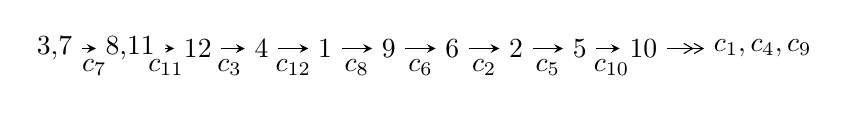
\begin{tikzpicture}[x=23pt, y=7pt]
	% node
	\node (A0) at (-1/8, 0) {3,7};
	\node (A1) at (17/16, 0) {8,11};
	\node (A2) at (17/8, 0) {12};
	\node (A3) at (25/8, 0) {4};
	\node (A4) at (33/8, 0) {1};
	\node (A5) at (41/8, 0) {9};
	\node (A6) at (49/8, 0) {6};
	\node (A7) at (57/8, 0) {2};
	\node (A8) at (65/8, 0) {5};
	\node (A9) at (73/8, 0) {10};
	\node (C1) at (1/2, -1) {$c_{7}$};
	\node (C2) at (13/8, -1) {$c_{11}$};
	\node (C3) at (21/8, -1) {$c_{3}$};
	\node (C4) at (29/8, -1) {$c_{12}$};
	\node (C5) at (37/8, -1) {$c_{8}$};
	\node (C6) at (45/8, -1) {$c_{6}$};
	\node (C7) at (53/8, -1) {$c_{2}$};
	\node (C8) at (61/8, -1) {$c_{5}$};
	\node (C9) at (69/8, -1) {$c_{10}$};
	\node (A10) at (11, 0) {$c_{1},c_{4},c_{9}$};

	% edge
	\draw[->,>=stealth]	
	(A0) edge (A1) (A1) edge (A2) (A2) edge (A3) (A3) edge (A4) (A4) edge (A5) (A5) edge (A6) (A6) edge (A7) (A7) edge (A8) (A8) edge (A9) ;
	\draw[->>,>={angle 60}]	
	(A9) edge (A10);
\end{tikzpicture} \\ 

\end{tabular} \\

\footnotetext{
The image of knot diagram is generated by the software ``\textbf{Draw programme}" developed by Andrew Bartholomew(\url{http://www.layer8.co.uk/maths/draw/index.htm\#Running-draw}), where we modified some parts for our purpose(\url{https://github.com/CATsTAILs/LinksPainter}).
}\phantom \\ \newline 
\centering \textbf{Ideals for irreducible components\footnotemark of $X_{\text{par}}$} 
 
\begin{align*}
I^u_{1}&=\langle 
-2.24498\times10^{1014} u^{129}-1.33093\times10^{1013} u^{128}+\cdots+9.28945\times10^{1015} b+1.16318\times10^{1016},\\
\phantom{I^u_{1}}&\phantom{= \langle  }-1.06674\times10^{1015} u^{129}-9.20458\times10^{1013} u^{128}+\cdots+1.32706\times10^{1015} a+4.44595\times10^{1016},\\
\phantom{I^u_{1}}&\phantom{= \langle  }u^{130}-2 u^{128}+\cdots-31 u+1\rangle \\
I^u_{2}&=\langle 
1.39792\times10^{34} u^{27}-2.23429\times10^{34} u^{26}+\cdots+6.97927\times10^{34} b-1.16827\times10^{34},\\
\phantom{I^u_{2}}&\phantom{= \langle  }-5.21376\times10^{33} u^{27}+5.87908\times10^{33} u^{26}+\cdots+6.97927\times10^{34} a-3.33304\times10^{34},\;u^{28}- u^{27}+\cdots+2 u^2-1\rangle \\
\\
\end{align*}
\raggedright * 2 irreducible components of $\dim_{\mathbb{C}}=0$, with total 158 representations.\\
\footnotetext{All coefficients of polynomials are rational numbers. But the coefficients are sometimes approximated in decimal forms when there is not enough margin.}
\newpage
\renewcommand{\arraystretch}{1}
\centering \section*{I. $I^u_{1}= \langle -2.24\times10^{1014} u^{129}-1.33\times10^{1013} u^{128}+\cdots+9.29\times10^{1015} b+1.16\times10^{1016},\;-1.07\times10^{1015} u^{129}-9.20\times10^{1013} u^{128}+\cdots+1.33\times10^{1015} a+4.45\times10^{1016},\;u^{130}-2 u^{128}+\cdots-31 u+1 \rangle$}
\flushleft \textbf{(i) Arc colorings}\\
\begin{tabular}{m{7pt} m{180pt} m{7pt} m{180pt} }
\flushright $a_{3}=$&$\begin{pmatrix}0\\u\end{pmatrix}$ \\
\flushright $a_{7}=$&$\begin{pmatrix}1\\0\end{pmatrix}$ \\
\flushright $a_{8}=$&$\begin{pmatrix}1\\- u^2\end{pmatrix}$ \\
\flushright $a_{11}=$&$\begin{pmatrix}0.803832 u^{129}+0.0693605 u^{128}+\cdots-301.493 u-33.5022\\0.0241670 u^{129}+0.00143273 u^{128}+\cdots-8.14510 u-1.25215\end{pmatrix}$ \\
\flushright $a_{12}=$&$\begin{pmatrix}0.779665 u^{129}+0.0679277 u^{128}+\cdots-293.348 u-32.2500\\0.0241670 u^{129}+0.00143273 u^{128}+\cdots-8.14510 u-1.25215\end{pmatrix}$ \\
\flushright $a_{4}=$&$\begin{pmatrix}0.503106 u^{129}+0.135213 u^{128}+\cdots-166.105 u-36.6631\\0.0850453 u^{129}-0.00933327 u^{128}+\cdots-18.2261 u-0.937790\end{pmatrix}$ \\
\flushright $a_{1}=$&$\begin{pmatrix}0.790741 u^{129}+0.0694749 u^{128}+\cdots-300.167 u-33.5701\\0.0222346 u^{129}+0.00215016 u^{128}+\cdots-8.18199 u-1.25060\end{pmatrix}$ \\
\flushright $a_{9}=$&$\begin{pmatrix}1.10939 u^{129}+0.0985816 u^{128}+\cdots-368.491 u-49.7757\\0.0499267 u^{129}-0.00557041 u^{128}+\cdots-7.45063 u-1.87644\end{pmatrix}$ \\
\flushright $a_{6}=$&$\begin{pmatrix}0.996665 u^{129}+0.0764168 u^{128}+\cdots-351.098 u-49.0893\\0.0588745 u^{129}-0.00862850 u^{128}+\cdots-9.17771 u-1.79165\end{pmatrix}$ \\
\flushright $a_{2}=$&$\begin{pmatrix}1.65851 u^{129}+0.120942 u^{128}+\cdots-524.027 u-72.9335\\0.0534113 u^{129}+0.00156281 u^{128}+\cdots-30.6408 u-2.23992\end{pmatrix}$ \\
\flushright $a_{5}=$&$\begin{pmatrix}0.359127 u^{129}+0.0172995 u^{128}+\cdots-246.271 u-42.4467\\0.0451233 u^{129}-0.0198763 u^{128}+\cdots-3.40264 u-1.63186\end{pmatrix}$ \\
\flushright $a_{10}=$&$\begin{pmatrix}-0.942279 u^{129}-0.0703869 u^{128}+\cdots+403.624 u+41.1454\\0.0496351 u^{129}-0.0147851 u^{128}+\cdots-2.48796 u+2.00130\end{pmatrix}$\\&\end{tabular}
\flushleft \textbf{(ii) Obstruction class $= -1$}\\~\\
\flushleft \textbf{(iii) Cusp Shapes $= 0.251625 u^{129}+0.0303260 u^{128}+\cdots-53.2435 u-5.10160$}\\~\\
\newpage\renewcommand{\arraystretch}{1}
\flushleft \textbf{(iv) u-Polynomials at the component}\newline \\
\begin{tabular}{m{50pt}|m{274pt}}
Crossings & \hspace{64pt}u-Polynomials at each crossing \\
\hline $$\begin{aligned}c_{1}\end{aligned}$$&$\begin{aligned}
&u^{130}+11 u^{129}+\cdots+1619394 u-1908844
\end{aligned}$\\
\hline $$\begin{aligned}c_{2}\end{aligned}$$&$\begin{aligned}
&u^{130}+3 u^{129}+\cdots+2106443 u+199853
\end{aligned}$\\
\hline $$\begin{aligned}c_{3}\end{aligned}$$&$\begin{aligned}
&u^{130}-3 u^{128}+\cdots-69 u+7
\end{aligned}$\\
\hline $$\begin{aligned}c_{4},c_{5},c_{9}\end{aligned}$$&$\begin{aligned}
&u^{130}-3 u^{129}+\cdots+229 u-29
\end{aligned}$\\
\hline $$\begin{aligned}c_{6},c_{11}\end{aligned}$$&$\begin{aligned}
&u^{130}- u^{129}+\cdots-346 u-28
\end{aligned}$\\
\hline $$\begin{aligned}c_{7}\end{aligned}$$&$\begin{aligned}
&u^{130}-2 u^{128}+\cdots-31 u+1
\end{aligned}$\\
\hline $$\begin{aligned}c_{8},c_{12}\end{aligned}$$&$\begin{aligned}
&u^{130}+u^{129}+\cdots+130501 u-12281
\end{aligned}$\\
\hline $$\begin{aligned}c_{10}\end{aligned}$$&$\begin{aligned}
&u^{130}+7 u^{129}+\cdots-32698791 u-1935199
\end{aligned}$\\
\hline
\end{tabular}\\~\\
\newpage\renewcommand{\arraystretch}{1}
\flushleft \textbf{(v) Riley Polynomials at the component}\newline \\
\begin{tabular}{m{50pt}|m{274pt}}
Crossings & \hspace{64pt}Riley Polynomials at each crossing \\
\hline $$\begin{aligned}c_{1}\end{aligned}$$&$\begin{aligned}
&y^{130}-23 y^{129}+\cdots-118783470217580 y+3643685416336
\end{aligned}$\\
\hline $$\begin{aligned}c_{2}\end{aligned}$$&$\begin{aligned}
&y^{130}+29 y^{129}+\cdots+1803493276335 y+39941221609
\end{aligned}$\\
\hline $$\begin{aligned}c_{3}\end{aligned}$$&$\begin{aligned}
&y^{130}-6 y^{129}+\cdots-6679 y+49
\end{aligned}$\\
\hline $$\begin{aligned}c_{4},c_{5},c_{9}\end{aligned}$$&$\begin{aligned}
&y^{130}+125 y^{129}+\cdots-59517 y+841
\end{aligned}$\\
\hline $$\begin{aligned}c_{6},c_{11}\end{aligned}$$&$\begin{aligned}
&y^{130}-97 y^{129}+\cdots-35996 y+784
\end{aligned}$\\
\hline $$\begin{aligned}c_{7}\end{aligned}$$&$\begin{aligned}
&y^{130}-4 y^{129}+\cdots-1573 y+1
\end{aligned}$\\
\hline $$\begin{aligned}c_{8},c_{12}\end{aligned}$$&$\begin{aligned}
&y^{130}-89 y^{129}+\cdots-4730278955 y+150822961
\end{aligned}$\\
\hline $$\begin{aligned}c_{10}\end{aligned}$$&$\begin{aligned}
&y^{130}-53 y^{129}+\cdots-307271885066539 y+3744995169601
\end{aligned}$\\
\hline
\end{tabular}\\~\\
\newpage\flushleft \textbf{(vi) Complex Volumes and Cusp Shapes}
$$\begin{array}{c|c|c}  
\text{Solutions to }I^u_{1}& \I (\text{vol} + \sqrt{-1}CS) & \text{Cusp shape}\\
 \hline 
\begin{aligned}
u &= \phantom{-}0.568518 + 0.818526 I \\
a &= \phantom{-}1.30537 + 0.68838 I \\
b &= \phantom{-}1.47617 - 0.47349 I\end{aligned}
 & -12.09710 + 0.66028 I & \phantom{-0.000000 } 0 \\ \hline\begin{aligned}
u &= \phantom{-}0.568518 - 0.818526 I \\
a &= \phantom{-}1.30537 - 0.68838 I \\
b &= \phantom{-}1.47617 + 0.47349 I\end{aligned}
 & -12.09710 - 0.66028 I & \phantom{-0.000000 } 0 \\ \hline\begin{aligned}
u &= -0.637610 + 0.794466 I \\
a &= \phantom{-}0.464149 - 0.108175 I \\
b &= \phantom{-}0.210670 + 0.855261 I\end{aligned}
 & -5.66679 - 1.84230 I & \phantom{-0.000000 } 0 \\ \hline\begin{aligned}
u &= -0.637610 - 0.794466 I \\
a &= \phantom{-}0.464149 + 0.108175 I \\
b &= \phantom{-}0.210670 - 0.855261 I\end{aligned}
 & -5.66679 + 1.84230 I & \phantom{-0.000000 } 0 \\ \hline\begin{aligned}
u &= \phantom{-}1.04253\phantom{ +0.000000I} \\
a &= -1.13091\phantom{ +0.000000I} \\
b &= \phantom{-}1.02886\phantom{ +0.000000I}\end{aligned}
 & \phantom{-}2.21961\phantom{ +0.000000I} & \phantom{-0.000000 } 0 \\ \hline\begin{aligned}
u &= \phantom{-}0.951082 + 0.430021 I \\
a &= -0.828807 + 0.377896 I \\
b &= -0.464152 - 0.648287 I\end{aligned}
 & \phantom{-}1.30389 + 1.17953 I & \phantom{-0.000000 } 0 \\ \hline\begin{aligned}
u &= \phantom{-}0.951082 - 0.430021 I \\
a &= -0.828807 - 0.377896 I \\
b &= -0.464152 + 0.648287 I\end{aligned}
 & \phantom{-}1.30389 - 1.17953 I & \phantom{-0.000000 } 0 \\ \hline\begin{aligned}
u &= -0.470392 + 0.933123 I \\
a &= \phantom{-}1.89360 - 0.36472 I \\
b &= \phantom{-}1.186250 + 0.305958 I\end{aligned}
 & -1.94110 - 4.24597 I & \phantom{-0.000000 } 0 \\ \hline\begin{aligned}
u &= -0.470392 - 0.933123 I \\
a &= \phantom{-}1.89360 + 0.36472 I \\
b &= \phantom{-}1.186250 - 0.305958 I\end{aligned}
 & -1.94110 + 4.24597 I & \phantom{-0.000000 } 0 \\ \hline\begin{aligned}
u &= \phantom{-}0.874780 + 0.584116 I \\
a &= -0.166962 - 0.175074 I \\
b &= -0.097138 + 1.104550 I\end{aligned}
 & \phantom{-}2.68104 + 3.43893 I & \phantom{-0.000000 } 0\\
 \hline 
 \end{array}$$\newpage$$\begin{array}{c|c|c}  
\text{Solutions to }I^u_{1}& \I (\text{vol} + \sqrt{-1}CS) & \text{Cusp shape}\\
 \hline 
\begin{aligned}
u &= \phantom{-}0.874780 - 0.584116 I \\
a &= -0.166962 + 0.175074 I \\
b &= -0.097138 - 1.104550 I\end{aligned}
 & \phantom{-}2.68104 - 3.43893 I & \phantom{-0.000000 } 0 \\ \hline\begin{aligned}
u &= -0.945830 + 0.024389 I \\
a &= -1.180790 - 0.402427 I \\
b &= \phantom{-}0.278518 + 0.568230 I\end{aligned}
 & -3.21381 + 5.65085 I & \phantom{-0.000000 } 0 \\ \hline\begin{aligned}
u &= -0.945830 - 0.024389 I \\
a &= -1.180790 + 0.402427 I \\
b &= \phantom{-}0.278518 - 0.568230 I\end{aligned}
 & -3.21381 - 5.65085 I & \phantom{-0.000000 } 0 \\ \hline\begin{aligned}
u &= \phantom{-}0.450456 + 0.953997 I \\
a &= -2.39991 - 0.39655 I \\
b &= -1.209660 + 0.279992 I\end{aligned}
 & -8.38195 + 6.60170 I & \phantom{-0.000000 } 0 \\ \hline\begin{aligned}
u &= \phantom{-}0.450456 - 0.953997 I \\
a &= -2.39991 + 0.39655 I \\
b &= -1.209660 - 0.279992 I\end{aligned}
 & -8.38195 - 6.60170 I & \phantom{-0.000000 } 0 \\ \hline\begin{aligned}
u &= \phantom{-}0.569234 + 0.750774 I \\
a &= \phantom{-}1.238770 - 0.612083 I \\
b &= \phantom{-}0.276603 - 0.175451 I\end{aligned}
 & -6.85078 - 2.81764 I & \phantom{-0.000000 } 0 \\ \hline\begin{aligned}
u &= \phantom{-}0.569234 - 0.750774 I \\
a &= \phantom{-}1.238770 + 0.612083 I \\
b &= \phantom{-}0.276603 + 0.175451 I\end{aligned}
 & -6.85078 + 2.81764 I & \phantom{-0.000000 } 0 \\ \hline\begin{aligned}
u &= -0.798627 + 0.487456 I \\
a &= \phantom{-}0.40101 - 1.67975 I \\
b &= \phantom{-}0.989295 + 0.553100 I\end{aligned}
 & -0.04628 - 5.21430 I & \phantom{-0.000000 } 0 \\ \hline\begin{aligned}
u &= -0.798627 - 0.487456 I \\
a &= \phantom{-}0.40101 + 1.67975 I \\
b &= \phantom{-}0.989295 - 0.553100 I\end{aligned}
 & -0.04628 + 5.21430 I & \phantom{-0.000000 } 0 \\ \hline\begin{aligned}
u &= -0.851565 + 0.673850 I \\
a &= \phantom{-}0.558040 + 0.104305 I \\
b &= -0.088096 + 0.586995 I\end{aligned}
 & -4.99906 - 3.32889 I & \phantom{-0.000000 } 0\\
 \hline 
 \end{array}$$\newpage$$\begin{array}{c|c|c}  
\text{Solutions to }I^u_{1}& \I (\text{vol} + \sqrt{-1}CS) & \text{Cusp shape}\\
 \hline 
\begin{aligned}
u &= -0.851565 - 0.673850 I \\
a &= \phantom{-}0.558040 - 0.104305 I \\
b &= -0.088096 - 0.586995 I\end{aligned}
 & -4.99906 + 3.32889 I & \phantom{-0.000000 } 0 \\ \hline\begin{aligned}
u &= -0.756818 + 0.797639 I \\
a &= \phantom{-}0.792094 - 1.069500 I \\
b &= \phantom{-}1.195650 + 0.047584 I\end{aligned}
 & -5.08072 - 1.54588 I & \phantom{-0.000000 } 0 \\ \hline\begin{aligned}
u &= -0.756818 - 0.797639 I \\
a &= \phantom{-}0.792094 + 1.069500 I \\
b &= \phantom{-}1.195650 - 0.047584 I\end{aligned}
 & -5.08072 + 1.54588 I & \phantom{-0.000000 } 0 \\ \hline\begin{aligned}
u &= -0.202487 + 1.081850 I \\
a &= \phantom{-}1.226540 + 0.006342 I \\
b &= \phantom{-}1.006010 + 0.676072 I\end{aligned}
 & -5.23300 - 3.00524 I & \phantom{-0.000000 } 0 \\ \hline\begin{aligned}
u &= -0.202487 - 1.081850 I \\
a &= \phantom{-}1.226540 - 0.006342 I \\
b &= \phantom{-}1.006010 - 0.676072 I\end{aligned}
 & -5.23300 + 3.00524 I & \phantom{-0.000000 } 0 \\ \hline\begin{aligned}
u &= \phantom{-}0.067821 + 0.892695 I \\
a &= \phantom{-}0.863538 + 0.730379 I \\
b &= -0.217358 + 0.116213 I\end{aligned}
 & \phantom{-}1.66983 + 3.99377 I & \phantom{-0.000000 } 0 \\ \hline\begin{aligned}
u &= \phantom{-}0.067821 - 0.892695 I \\
a &= \phantom{-}0.863538 - 0.730379 I \\
b &= -0.217358 - 0.116213 I\end{aligned}
 & \phantom{-}1.66983 - 3.99377 I & \phantom{-0.000000 } 0 \\ \hline\begin{aligned}
u &= -0.996392 + 0.543578 I \\
a &= \phantom{-}0.529252 + 0.119952 I \\
b &= \phantom{-}0.267432 - 0.768275 I\end{aligned}
 & \phantom{-}4.80286 - 2.81007 I & \phantom{-0.000000 } 0 \\ \hline\begin{aligned}
u &= -0.996392 - 0.543578 I \\
a &= \phantom{-}0.529252 - 0.119952 I \\
b &= \phantom{-}0.267432 + 0.768275 I\end{aligned}
 & \phantom{-}4.80286 + 2.81007 I & \phantom{-0.000000 } 0 \\ \hline\begin{aligned}
u &= \phantom{-}0.360758 + 1.079490 I \\
a &= -1.278930 - 0.330588 I \\
b &= -0.997476 + 0.349523 I\end{aligned}
 & -1.40422 + 1.99566 I & \phantom{-0.000000 } 0\\
 \hline 
 \end{array}$$\newpage$$\begin{array}{c|c|c}  
\text{Solutions to }I^u_{1}& \I (\text{vol} + \sqrt{-1}CS) & \text{Cusp shape}\\
 \hline 
\begin{aligned}
u &= \phantom{-}0.360758 - 1.079490 I \\
a &= -1.278930 + 0.330588 I \\
b &= -0.997476 - 0.349523 I\end{aligned}
 & -1.40422 - 1.99566 I & \phantom{-0.000000 } 0 \\ \hline\begin{aligned}
u &= \phantom{-}0.827739 + 0.205538 I \\
a &= \phantom{-}0.99749 - 1.21579 I \\
b &= -0.588180 + 0.543593 I\end{aligned}
 & \phantom{-}2.26163 - 0.80769 I & \phantom{-0.000000 } 0 \\ \hline\begin{aligned}
u &= \phantom{-}0.827739 - 0.205538 I \\
a &= \phantom{-}0.99749 + 1.21579 I \\
b &= -0.588180 - 0.543593 I\end{aligned}
 & \phantom{-}2.26163 + 0.80769 I & \phantom{-0.000000 } 0 \\ \hline\begin{aligned}
u &= \phantom{-}0.411826 + 0.745086 I \\
a &= -1.32426 - 1.85371 I \\
b &= -1.286230 + 0.045954 I\end{aligned}
 & -11.67270 + 2.83151 I & \phantom{-0.000000 } 0 \\ \hline\begin{aligned}
u &= \phantom{-}0.411826 - 0.745086 I \\
a &= -1.32426 + 1.85371 I \\
b &= -1.286230 - 0.045954 I\end{aligned}
 & -11.67270 - 2.83151 I & \phantom{-0.000000 } 0 \\ \hline\begin{aligned}
u &= \phantom{-}0.992024 + 0.581122 I \\
a &= -0.527207 - 0.093630 I \\
b &= -0.243157 - 0.929089 I\end{aligned}
 & \phantom{-}0.13818 + 4.79899 I & \phantom{-0.000000 } 0 \\ \hline\begin{aligned}
u &= \phantom{-}0.992024 - 0.581122 I \\
a &= -0.527207 + 0.093630 I \\
b &= -0.243157 + 0.929089 I\end{aligned}
 & \phantom{-}0.13818 - 4.79899 I & \phantom{-0.000000 } 0 \\ \hline\begin{aligned}
u &= \phantom{-}0.813245 + 0.825477 I \\
a &= -1.46553 + 0.09382 I \\
b &= -1.378720 + 0.191672 I\end{aligned}
 & -2.61977 + 3.30642 I & \phantom{-0.000000 } 0 \\ \hline\begin{aligned}
u &= \phantom{-}0.813245 - 0.825477 I \\
a &= -1.46553 - 0.09382 I \\
b &= -1.378720 - 0.191672 I\end{aligned}
 & -2.61977 - 3.30642 I & \phantom{-0.000000 } 0 \\ \hline\begin{aligned}
u &= -0.784196 + 0.868456 I \\
a &= -1.229760 + 0.495103 I \\
b &= -1.45433 - 0.47406 I\end{aligned}
 & -5.35695 - 4.09374 I & \phantom{-0.000000 } 0\\
 \hline 
 \end{array}$$\newpage$$\begin{array}{c|c|c}  
\text{Solutions to }I^u_{1}& \I (\text{vol} + \sqrt{-1}CS) & \text{Cusp shape}\\
 \hline 
\begin{aligned}
u &= -0.784196 - 0.868456 I \\
a &= -1.229760 - 0.495103 I \\
b &= -1.45433 + 0.47406 I\end{aligned}
 & -5.35695 + 4.09374 I & \phantom{-0.000000 } 0 \\ \hline\begin{aligned}
u &= -0.988827 + 0.641667 I \\
a &= \phantom{-}0.0996686 - 0.0541932 I \\
b &= \phantom{-}0.168601 + 1.111570 I\end{aligned}
 & \phantom{-}4.12867 - 8.76175 I & \phantom{-0.000000 } 0 \\ \hline\begin{aligned}
u &= -0.988827 - 0.641667 I \\
a &= \phantom{-}0.0996686 + 0.0541932 I \\
b &= \phantom{-}0.168601 - 1.111570 I\end{aligned}
 & \phantom{-}4.12867 + 8.76175 I & \phantom{-0.000000 } 0 \\ \hline\begin{aligned}
u &= \phantom{-}0.211629 + 0.783048 I \\
a &= -1.44980 + 0.01856 I \\
b &= -1.32973 + 0.56352 I\end{aligned}
 & -1.98456 + 2.68666 I & \phantom{-0.000000 } 0 \\ \hline\begin{aligned}
u &= \phantom{-}0.211629 - 0.783048 I \\
a &= -1.44980 - 0.01856 I \\
b &= -1.32973 - 0.56352 I\end{aligned}
 & -1.98456 - 2.68666 I & \phantom{-0.000000 } 0 \\ \hline\begin{aligned}
u &= -0.949576 + 0.735901 I \\
a &= -0.59807 + 1.50031 I \\
b &= -1.100920 - 0.089462 I\end{aligned}
 & -0.60698 - 4.59108 I & \phantom{-0.000000 } 0 \\ \hline\begin{aligned}
u &= -0.949576 - 0.735901 I \\
a &= -0.59807 - 1.50031 I \\
b &= -1.100920 + 0.089462 I\end{aligned}
 & -0.60698 + 4.59108 I & \phantom{-0.000000 } 0 \\ \hline\begin{aligned}
u &= \phantom{-}0.543250 + 1.084010 I \\
a &= \phantom{-}2.04031 + 1.44697 I \\
b &= \phantom{-}1.222590 - 0.032319 I\end{aligned}
 & -8.13441 + 6.95442 I & \phantom{-0.000000 } 0 \\ \hline\begin{aligned}
u &= \phantom{-}0.543250 - 1.084010 I \\
a &= \phantom{-}2.04031 - 1.44697 I \\
b &= \phantom{-}1.222590 + 0.032319 I\end{aligned}
 & -8.13441 - 6.95442 I & \phantom{-0.000000 } 0 \\ \hline\begin{aligned}
u &= -0.776691\phantom{ +0.000000I} \\
a &= \phantom{-}1.47696\phantom{ +0.000000I} \\
b &= \phantom{-}1.58587\phantom{ +0.000000I}\end{aligned}
 & \phantom{-}0.811342\phantom{ +0.000000I} & \phantom{-}10.5810\phantom{ +0.000000I}\\
 \hline 
 \end{array}$$\newpage$$\begin{array}{c|c|c}  
\text{Solutions to }I^u_{1}& \I (\text{vol} + \sqrt{-1}CS) & \text{Cusp shape}\\
 \hline 
\begin{aligned}
u &= \phantom{-}0.063893 + 0.753553 I \\
a &= \phantom{-}1.44833 + 0.06651 I \\
b &= \phantom{-}1.37010 + 0.77618 I\end{aligned}
 & -8.18877 - 4.30023 I & -13.84345 + 0. I\phantom{ +0.000000I} \\ \hline\begin{aligned}
u &= \phantom{-}0.063893 - 0.753553 I \\
a &= \phantom{-}1.44833 - 0.06651 I \\
b &= \phantom{-}1.37010 - 0.77618 I\end{aligned}
 & -8.18877 + 4.30023 I & -13.84345 + 0. I\phantom{ +0.000000I} \\ \hline\begin{aligned}
u &= \phantom{-}1.042030 + 0.709443 I \\
a &= -0.1004160 + 0.0355801 I \\
b &= -0.191526 + 1.110900 I\end{aligned}
 & -1.87169 + 13.08240 I & \phantom{-0.000000 } 0 \\ \hline\begin{aligned}
u &= \phantom{-}1.042030 - 0.709443 I \\
a &= -0.1004160 - 0.0355801 I \\
b &= -0.191526 - 1.110900 I\end{aligned}
 & -1.87169 - 13.08240 I & \phantom{-0.000000 } 0 \\ \hline\begin{aligned}
u &= \phantom{-}0.100950 + 1.292880 I \\
a &= -0.700789 + 0.448440 I \\
b &= \phantom{-}0.011735 + 0.195257 I\end{aligned}
 & -4.55877 - 7.16989 I & \phantom{-0.000000 } 0 \\ \hline\begin{aligned}
u &= \phantom{-}0.100950 - 1.292880 I \\
a &= -0.700789 - 0.448440 I \\
b &= \phantom{-}0.011735 - 0.195257 I\end{aligned}
 & -4.55877 + 7.16989 I & \phantom{-0.000000 } 0 \\ \hline\begin{aligned}
u &= \phantom{-}0.461286 + 0.496352 I \\
a &= -0.905894 - 0.505575 I \\
b &= \phantom{-}0.386005 + 0.621122 I\end{aligned}
 & \phantom{-}1.59323 + 0.61502 I & \phantom{-}3.23997 + 0.71765 I \\ \hline\begin{aligned}
u &= \phantom{-}0.461286 - 0.496352 I \\
a &= -0.905894 + 0.505575 I \\
b &= \phantom{-}0.386005 - 0.621122 I\end{aligned}
 & \phantom{-}1.59323 - 0.61502 I & \phantom{-}3.23997 - 0.71765 I \\ \hline\begin{aligned}
u &= \phantom{-}0.832812 + 1.049160 I \\
a &= \phantom{-}1.308550 + 0.391317 I \\
b &= \phantom{-}1.43005 - 0.49799 I\end{aligned}
 & -5.31453 + 8.79742 I & \phantom{-0.000000 } 0 \\ \hline\begin{aligned}
u &= \phantom{-}0.832812 - 1.049160 I \\
a &= \phantom{-}1.308550 - 0.391317 I \\
b &= \phantom{-}1.43005 + 0.49799 I\end{aligned}
 & -5.31453 - 8.79742 I & \phantom{-0.000000 } 0\\
 \hline 
 \end{array}$$\newpage$$\begin{array}{c|c|c}  
\text{Solutions to }I^u_{1}& \I (\text{vol} + \sqrt{-1}CS) & \text{Cusp shape}\\
 \hline 
\begin{aligned}
u &= \phantom{-}1.183160 + 0.633725 I \\
a &= -0.1075880 + 0.0836287 I \\
b &= \phantom{-}0.027792 - 0.654590 I\end{aligned}
 & \phantom{-}5.04522 + 2.01937 I & \phantom{-0.000000 } 0 \\ \hline\begin{aligned}
u &= \phantom{-}1.183160 - 0.633725 I \\
a &= -0.1075880 - 0.0836287 I \\
b &= \phantom{-}0.027792 + 0.654590 I\end{aligned}
 & \phantom{-}5.04522 - 2.01937 I & \phantom{-0.000000 } 0 \\ \hline\begin{aligned}
u &= \phantom{-}0.607463 + 0.245216 I \\
a &= -0.337863 - 0.096883 I \\
b &= \phantom{-}0.230514 + 0.593673 I\end{aligned}
 & \phantom{-}1.045300 + 0.722902 I & \phantom{-}7.28787 - 2.21685 I \\ \hline\begin{aligned}
u &= \phantom{-}0.607463 - 0.245216 I \\
a &= -0.337863 + 0.096883 I \\
b &= \phantom{-}0.230514 - 0.593673 I\end{aligned}
 & \phantom{-}1.045300 - 0.722902 I & \phantom{-}7.28787 + 2.21685 I \\ \hline\begin{aligned}
u &= \phantom{-}0.886717 + 1.019400 I \\
a &= -1.41413 - 0.85934 I \\
b &= -1.338820 + 0.426017 I\end{aligned}
 & -10.31820 + 6.44691 I & \phantom{-0.000000 } 0 \\ \hline\begin{aligned}
u &= \phantom{-}0.886717 - 1.019400 I \\
a &= -1.41413 + 0.85934 I \\
b &= -1.338820 - 0.426017 I\end{aligned}
 & -10.31820 - 6.44691 I & \phantom{-0.000000 } 0 \\ \hline\begin{aligned}
u &= -1.292280 + 0.415632 I \\
a &= \phantom{-}0.141753 - 0.071946 I \\
b &= -0.077916 - 0.749294 I\end{aligned}
 & \phantom{-}0.772853 + 0.161579 I & \phantom{-0.000000 } 0 \\ \hline\begin{aligned}
u &= -1.292280 - 0.415632 I \\
a &= \phantom{-}0.141753 + 0.071946 I \\
b &= -0.077916 + 0.749294 I\end{aligned}
 & \phantom{-}0.772853 - 0.161579 I & \phantom{-0.000000 } 0 \\ \hline\begin{aligned}
u &= -0.783163 + 1.109200 I \\
a &= -1.086870 + 0.388891 I \\
b &= -1.226260 + 0.124123 I\end{aligned}
 & -3.06879 + 1.51869 I & \phantom{-0.000000 } 0 \\ \hline\begin{aligned}
u &= -0.783163 - 1.109200 I \\
a &= -1.086870 - 0.388891 I \\
b &= -1.226260 - 0.124123 I\end{aligned}
 & -3.06879 - 1.51869 I & \phantom{-0.000000 } 0\\
 \hline 
 \end{array}$$\newpage$$\begin{array}{c|c|c}  
\text{Solutions to }I^u_{1}& \I (\text{vol} + \sqrt{-1}CS) & \text{Cusp shape}\\
 \hline 
\begin{aligned}
u &= \phantom{-}0.387153 + 0.503535 I \\
a &= -0.067295 - 0.366604 I \\
b &= \phantom{-}0.141722 - 1.343650 I\end{aligned}
 & -6.80625 + 6.00852 I & -6.5984 - 12.6049 I \\ \hline\begin{aligned}
u &= \phantom{-}0.387153 - 0.503535 I \\
a &= -0.067295 + 0.366604 I \\
b &= \phantom{-}0.141722 + 1.343650 I\end{aligned}
 & -6.80625 - 6.00852 I & -6.5984 + 12.6049 I \\ \hline\begin{aligned}
u &= -0.771931 + 1.160580 I \\
a &= -1.38549 + 0.35998 I \\
b &= -1.43485 - 0.52823 I\end{aligned}
 & -11.7969 - 12.2543 I & \phantom{-0.000000 } 0 \\ \hline\begin{aligned}
u &= -0.771931 - 1.160580 I \\
a &= -1.38549 - 0.35998 I \\
b &= -1.43485 + 0.52823 I\end{aligned}
 & -11.7969 + 12.2543 I & \phantom{-0.000000 } 0 \\ \hline\begin{aligned}
u &= -0.185381 + 0.575056 I \\
a &= -0.95437 - 1.07132 I \\
b &= -0.151887 + 0.044542 I\end{aligned}
 & -1.33016 + 0.97965 I & -5.31368 - 0.58456 I \\ \hline\begin{aligned}
u &= -0.185381 - 0.575056 I \\
a &= -0.95437 + 1.07132 I \\
b &= -0.151887 - 0.044542 I\end{aligned}
 & -1.33016 - 0.97965 I & -5.31368 + 0.58456 I \\ \hline\begin{aligned}
u &= -0.495512 + 0.249127 I \\
a &= \phantom{-}0.005156 - 0.155426 I \\
b &= -0.376065 - 1.159250 I\end{aligned}
 & -0.00070 - 2.98592 I & \phantom{-}5.8038 + 13.7955 I \\ \hline\begin{aligned}
u &= -0.495512 - 0.249127 I \\
a &= \phantom{-}0.005156 + 0.155426 I \\
b &= -0.376065 + 1.159250 I\end{aligned}
 & -0.00070 + 2.98592 I & \phantom{-}5.8038 - 13.7955 I \\ \hline\begin{aligned}
u &= \phantom{-}0.412006 + 0.348495 I \\
a &= -2.81811 + 0.17207 I \\
b &= -1.004020 + 0.268799 I\end{aligned}
 & -2.21129 + 3.77738 I & \phantom{-}0.40260 - 4.14688 I \\ \hline\begin{aligned}
u &= \phantom{-}0.412006 - 0.348495 I \\
a &= -2.81811 - 0.17207 I \\
b &= -1.004020 - 0.268799 I\end{aligned}
 & -2.21129 - 3.77738 I & \phantom{-}0.40260 + 4.14688 I\\
 \hline 
 \end{array}$$\newpage$$\begin{array}{c|c|c}  
\text{Solutions to }I^u_{1}& \I (\text{vol} + \sqrt{-1}CS) & \text{Cusp shape}\\
 \hline 
\begin{aligned}
u &= -0.519885 + 0.092491 I \\
a &= -0.208154 + 0.540120 I \\
b &= -1.097060 - 0.772163 I\end{aligned}
 & -0.60445 - 3.18290 I & \phantom{-}7.51976 - 6.77683 I \\ \hline\begin{aligned}
u &= -0.519885 - 0.092491 I \\
a &= -0.208154 - 0.540120 I \\
b &= -1.097060 + 0.772163 I\end{aligned}
 & -0.60445 + 3.18290 I & \phantom{-}7.51976 + 6.77683 I \\ \hline\begin{aligned}
u &= -1.16519 + 0.92556 I \\
a &= -0.104464 + 0.206239 I \\
b &= -0.103477 - 0.485368 I\end{aligned}
 & \phantom{-}1.27402 - 3.96073 I & \phantom{-0.000000 } 0 \\ \hline\begin{aligned}
u &= -1.16519 - 0.92556 I \\
a &= -0.104464 - 0.206239 I \\
b &= -0.103477 + 0.485368 I\end{aligned}
 & \phantom{-}1.27402 + 3.96073 I & \phantom{-0.000000 } 0 \\ \hline\begin{aligned}
u &= -1.14397 + 0.96921 I \\
a &= \phantom{-}1.205010 - 0.652882 I \\
b &= \phantom{-}1.38530 + 0.50548 I\end{aligned}
 & -1.94816 - 9.09119 I & \phantom{-0.000000 } 0 \\ \hline\begin{aligned}
u &= -1.14397 - 0.96921 I \\
a &= \phantom{-}1.205010 + 0.652882 I \\
b &= \phantom{-}1.38530 - 0.50548 I\end{aligned}
 & -1.94816 + 9.09119 I & \phantom{-0.000000 } 0 \\ \hline\begin{aligned}
u &= -0.52765 + 1.40725 I \\
a &= \phantom{-}1.074260 - 0.512404 I \\
b &= \phantom{-}0.957876 + 0.073390 I\end{aligned}
 & -5.44235 - 0.12690 I & \phantom{-0.000000 } 0 \\ \hline\begin{aligned}
u &= -0.52765 - 1.40725 I \\
a &= \phantom{-}1.074260 + 0.512404 I \\
b &= \phantom{-}0.957876 - 0.073390 I\end{aligned}
 & -5.44235 + 0.12690 I & \phantom{-0.000000 } 0 \\ \hline\begin{aligned}
u &= -0.420068 + 0.241749 I \\
a &= -1.175000 - 0.342744 I \\
b &= -1.28386 + 1.01152 I\end{aligned}
 & -4.84120 - 6.22354 I & \phantom{-}5.4710 + 14.7902 I \\ \hline\begin{aligned}
u &= -0.420068 - 0.241749 I \\
a &= -1.175000 + 0.342744 I \\
b &= -1.28386 - 1.01152 I\end{aligned}
 & -4.84120 + 6.22354 I & \phantom{-}5.4710 - 14.7902 I\\
 \hline 
 \end{array}$$\newpage$$\begin{array}{c|c|c}  
\text{Solutions to }I^u_{1}& \I (\text{vol} + \sqrt{-1}CS) & \text{Cusp shape}\\
 \hline 
\begin{aligned}
u &= \phantom{-}0.422698 + 0.095404 I \\
a &= \phantom{-}0.705862 - 0.295463 I \\
b &= \phantom{-}1.11556 + 1.11797 I\end{aligned}
 & \phantom{-}1.22229 + 1.85561 I & \phantom{-}22.0787 - 10.1963 I \\ \hline\begin{aligned}
u &= \phantom{-}0.422698 - 0.095404 I \\
a &= \phantom{-}0.705862 + 0.295463 I \\
b &= \phantom{-}1.11556 - 1.11797 I\end{aligned}
 & \phantom{-}1.22229 - 1.85561 I & \phantom{-}22.0787 + 10.1963 I \\ \hline\begin{aligned}
u &= -1.30242 + 0.98890 I \\
a &= -0.792237 + 0.650634 I \\
b &= -1.067590 - 0.224668 I\end{aligned}
 & -0.30081 - 4.46992 I & \phantom{-0.000000 } 0 \\ \hline\begin{aligned}
u &= -1.30242 - 0.98890 I \\
a &= -0.792237 - 0.650634 I \\
b &= -1.067590 + 0.224668 I\end{aligned}
 & -0.30081 + 4.46992 I & \phantom{-0.000000 } 0 \\ \hline\begin{aligned}
u &= \phantom{-}1.23838 + 1.07050 I \\
a &= -1.258080 - 0.531794 I \\
b &= -1.41627 + 0.49751 I\end{aligned}
 & -0.8149 + 14.4271 I & \phantom{-0.000000 } 0 \\ \hline\begin{aligned}
u &= \phantom{-}1.23838 - 1.07050 I \\
a &= -1.258080 + 0.531794 I \\
b &= -1.41627 - 0.49751 I\end{aligned}
 & -0.8149 - 14.4271 I & \phantom{-0.000000 } 0 \\ \hline\begin{aligned}
u &= -0.293653 + 0.069234 I \\
a &= \phantom{-}3.55119 + 3.51423 I \\
b &= \phantom{-}0.796509 - 0.134342 I\end{aligned}
 & \phantom{-}2.42862 + 0.45229 I & \phantom{-}4.76661 - 2.11342 I \\ \hline\begin{aligned}
u &= -0.293653 - 0.069234 I \\
a &= \phantom{-}3.55119 - 3.51423 I \\
b &= \phantom{-}0.796509 + 0.134342 I\end{aligned}
 & \phantom{-}2.42862 - 0.45229 I & \phantom{-}4.76661 + 2.11342 I \\ \hline\begin{aligned}
u &= \phantom{-}1.39175 + 0.98851 I \\
a &= -0.740426 - 0.493712 I \\
b &= -1.148850 - 0.051129 I\end{aligned}
 & -3.96210 - 1.34417 I & \phantom{-0.000000 } 0 \\ \hline\begin{aligned}
u &= \phantom{-}1.39175 - 0.98851 I \\
a &= -0.740426 + 0.493712 I \\
b &= -1.148850 + 0.051129 I\end{aligned}
 & -3.96210 + 1.34417 I & \phantom{-0.000000 } 0\\
 \hline 
 \end{array}$$\newpage$$\begin{array}{c|c|c}  
\text{Solutions to }I^u_{1}& \I (\text{vol} + \sqrt{-1}CS) & \text{Cusp shape}\\
 \hline 
\begin{aligned}
u &= -1.26021 + 1.16288 I \\
a &= \phantom{-}1.319990 - 0.482391 I \\
b &= \phantom{-}1.42923 + 0.48933 I\end{aligned}
 & -6.9416 - 18.7247 I & \phantom{-0.000000 } 0 \\ \hline\begin{aligned}
u &= -1.26021 - 1.16288 I \\
a &= \phantom{-}1.319990 + 0.482391 I \\
b &= \phantom{-}1.42923 - 0.48933 I\end{aligned}
 & -6.9416 + 18.7247 I & \phantom{-0.000000 } 0 \\ \hline\begin{aligned}
u &= \phantom{-}1.45814 + 0.99541 I \\
a &= \phantom{-}1.038330 + 0.232523 I \\
b &= \phantom{-}1.252460 + 0.129503 I\end{aligned}
 & -9.12657 + 0.95203 I & \phantom{-0.000000 } 0 \\ \hline\begin{aligned}
u &= \phantom{-}1.45814 - 0.99541 I \\
a &= \phantom{-}1.038330 - 0.232523 I \\
b &= \phantom{-}1.252460 - 0.129503 I\end{aligned}
 & -9.12657 - 0.95203 I & \phantom{-0.000000 } 0 \\ \hline\begin{aligned}
u &= \phantom{-}0.210588 + 0.062546 I \\
a &= \phantom{-}8.30722 + 7.91597 I \\
b &= \phantom{-}1.088860 - 0.276135 I\end{aligned}
 & -5.49689 + 8.93624 I & \phantom{-}1.05657 - 9.91092 I \\ \hline\begin{aligned}
u &= \phantom{-}0.210588 - 0.062546 I \\
a &= \phantom{-}8.30722 - 7.91597 I \\
b &= \phantom{-}1.088860 + 0.276135 I\end{aligned}
 & -5.49689 - 8.93624 I & \phantom{-}1.05657 + 9.91092 I \\ \hline\begin{aligned}
u &= -1.78051\phantom{ +0.000000I} \\
a &= \phantom{-}0.639192\phantom{ +0.000000I} \\
b &= \phantom{-}1.34270\phantom{ +0.000000I}\end{aligned}
 & -4.06041\phantom{ +0.000000I} & \phantom{-0.000000 } 0 \\ \hline\begin{aligned}
u &= -0.178443 + 0.120032 I \\
a &= \phantom{-}4.61817 - 8.10142 I \\
b &= -0.896347 + 0.294156 I\end{aligned}
 & \phantom{-}1.53512 + 4.48092 I & \phantom{-}6.80496 - 6.48563 I \\ \hline\begin{aligned}
u &= -0.178443 - 0.120032 I \\
a &= \phantom{-}4.61817 + 8.10142 I \\
b &= -0.896347 - 0.294156 I\end{aligned}
 & \phantom{-}1.53512 - 4.48092 I & \phantom{-}6.80496 + 6.48563 I \\ \hline\begin{aligned}
u &= \phantom{-}1.33776 + 1.22497 I \\
a &= \phantom{-}1.039230 + 0.354705 I \\
b &= \phantom{-}1.137430 - 0.374234 I\end{aligned}
 & \phantom{-}2.12244 + 7.00804 I & \phantom{-0.000000 } 0\\
 \hline 
 \end{array}$$\newpage$$\begin{array}{c|c|c}  
\text{Solutions to }I^u_{1}& \I (\text{vol} + \sqrt{-1}CS) & \text{Cusp shape}\\
 \hline 
\begin{aligned}
u &= \phantom{-}1.33776 - 1.22497 I \\
a &= \phantom{-}1.039230 - 0.354705 I \\
b &= \phantom{-}1.137430 + 0.374234 I\end{aligned}
 & \phantom{-}2.12244 - 7.00804 I & \phantom{-0.000000 } 0 \\ \hline\begin{aligned}
u &= -0.088296 + 0.152527 I \\
a &= \phantom{-}4.97308 + 4.88599 I \\
b &= \phantom{-}1.48620 - 0.09686 I\end{aligned}
 & -6.31465 - 0.78917 I & -6.24217 - 0.30715 I \\ \hline\begin{aligned}
u &= -0.088296 - 0.152527 I \\
a &= \phantom{-}4.97308 - 4.88599 I \\
b &= \phantom{-}1.48620 + 0.09686 I\end{aligned}
 & -6.31465 + 0.78917 I & -6.24217 + 0.30715 I \\ \hline\begin{aligned}
u &= -1.32067 + 1.29312 I \\
a &= -1.090110 + 0.238999 I \\
b &= -1.168530 - 0.457287 I\end{aligned}
 & -2.77584 - 9.74851 I & \phantom{-0.000000 } 0 \\ \hline\begin{aligned}
u &= -1.32067 - 1.29312 I \\
a &= -1.090110 - 0.238999 I \\
b &= -1.168530 + 0.457287 I\end{aligned}
 & -2.77584 + 9.74851 I & \phantom{-0.000000 } 0 \\ \hline\begin{aligned}
u &= \phantom{-}0.61897 + 1.76307 I \\
a &= \phantom{-}1.203580 + 0.294382 I \\
b &= \phantom{-}1.233020 + 0.136176 I\end{aligned}
 & -2.46866 - 5.31459 I & \phantom{-0.000000 } 0 \\ \hline\begin{aligned}
u &= \phantom{-}0.61897 - 1.76307 I \\
a &= \phantom{-}1.203580 - 0.294382 I \\
b &= \phantom{-}1.233020 - 0.136176 I\end{aligned}
 & -2.46866 + 5.31459 I & \phantom{-0.000000 } 0 \\ \hline\begin{aligned}
u &= -1.28788 + 1.36468 I \\
a &= -1.36172 + 0.40287 I \\
b &= -1.278860 - 0.292862 I\end{aligned}
 & \phantom{-}0.99532 - 5.52281 I & \phantom{-0.000000 } 0 \\ \hline\begin{aligned}
u &= -1.28788 - 1.36468 I \\
a &= -1.36172 - 0.40287 I \\
b &= -1.278860 + 0.292862 I\end{aligned}
 & \phantom{-}0.99532 + 5.52281 I & \phantom{-0.000000 } 0 \\ \hline\begin{aligned}
u &= \phantom{-}1.16983 + 1.50893 I \\
a &= \phantom{-}1.53578 + 0.45763 I \\
b &= \phantom{-}1.314610 - 0.244974 I\end{aligned}
 & -3.16990 + 6.81082 I & \phantom{-0.000000 } 0\\
 \hline 
 \end{array}$$\newpage$$\begin{array}{c|c|c}  
\text{Solutions to }I^u_{1}& \I (\text{vol} + \sqrt{-1}CS) & \text{Cusp shape}\\
 \hline 
\begin{aligned}
u &= \phantom{-}1.16983 - 1.50893 I \\
a &= \phantom{-}1.53578 - 0.45763 I \\
b &= \phantom{-}1.314610 + 0.244974 I\end{aligned}
 & -3.16990 - 6.81082 I & \phantom{-0.000000 } 0 \\ \hline\begin{aligned}
u &= \phantom{-}1.93101 + 0.10644 I \\
a &= -0.712713 - 0.091674 I \\
b &= -1.341950 - 0.115937 I\end{aligned}
 & -8.40996 + 3.46860 I & \phantom{-0.000000 } 0 \\ \hline\begin{aligned}
u &= \phantom{-}1.93101 - 0.10644 I \\
a &= -0.712713 + 0.091674 I \\
b &= -1.341950 + 0.115937 I\end{aligned}
 & -8.40996 - 3.46860 I & \phantom{-0.000000 } 0 \\ \hline\begin{aligned}
u &= \phantom{-}1.44864 + 1.31043 I \\
a &= \phantom{-}1.325420 + 0.262887 I \\
b &= \phantom{-}1.306550 - 0.331865 I\end{aligned}
 & -3.54424 + 3.76653 I & \phantom{-0.000000 } 0 \\ \hline\begin{aligned}
u &= \phantom{-}1.44864 - 1.31043 I \\
a &= \phantom{-}1.325420 - 0.262887 I \\
b &= \phantom{-}1.306550 + 0.331865 I\end{aligned}
 & -3.54424 - 3.76653 I & \phantom{-0.000000 } 0 \\ \hline\begin{aligned}
u &= \phantom{-}0.0256857\phantom{ +0.000000I} \\
a &= -41.0569\phantom{ +0.000000I} \\
b &= -1.43304\phantom{ +0.000000I}\end{aligned}
 & -1.59020\phantom{ +0.000000I} & -6.43260\phantom{ +0.000000I} \\ \hline\begin{aligned}
u &= -1.83014 + 1.05812 I \\
a &= \phantom{-}0.789120 - 0.368630 I \\
b &= \phantom{-}1.150740 - 0.110794 I\end{aligned}
 & -9.33600 + 4.11530 I & \phantom{-0.000000 } 0 \\ \hline\begin{aligned}
u &= -1.83014 - 1.05812 I \\
a &= \phantom{-}0.789120 + 0.368630 I \\
b &= \phantom{-}1.150740 + 0.110794 I\end{aligned}
 & -9.33600 - 4.11530 I & \phantom{-0.000000 } 0 \\ \hline\begin{aligned}
u &= -0.85403 + 2.15944 I \\
a &= -1.192310 + 0.243332 I \\
b &= -1.232990 + 0.134244 I\end{aligned}
 & -8.26846 + 8.61335 I & \phantom{-0.000000 } 0 \\ \hline\begin{aligned}
u &= -0.85403 - 2.15944 I \\
a &= -1.192310 - 0.243332 I \\
b &= -1.232990 - 0.134244 I\end{aligned}
 & -8.26846 - 8.61335 I & \phantom{-0.000000 } 0\\
 \hline 
 \end{array}$$\newpage\newpage\renewcommand{\arraystretch}{1}
\centering \section*{II. $I^u_{2}= \langle 1.40\times10^{34} u^{27}-2.23\times10^{34} u^{26}+\cdots+6.98\times10^{34} b-1.17\times10^{34},\;-5.21\times10^{33} u^{27}+5.88\times10^{33} u^{26}+\cdots+6.98\times10^{34} a-3.33\times10^{34},\;u^{28}- u^{27}+\cdots+2 u^2-1 \rangle$}
\flushleft \textbf{(i) Arc colorings}\\
\begin{tabular}{m{7pt} m{180pt} m{7pt} m{180pt} }
\flushright $a_{3}=$&$\begin{pmatrix}0\\u\end{pmatrix}$ \\
\flushright $a_{7}=$&$\begin{pmatrix}1\\0\end{pmatrix}$ \\
\flushright $a_{8}=$&$\begin{pmatrix}1\\- u^2\end{pmatrix}$ \\
\flushright $a_{11}=$&$\begin{pmatrix}0.0747036 u^{27}-0.0842364 u^{26}+\cdots+0.676191 u+0.477563\\-0.200297 u^{27}+0.320133 u^{26}+\cdots-2.64575 u+0.167391\end{pmatrix}$ \\
\flushright $a_{12}=$&$\begin{pmatrix}0.275000 u^{27}-0.404370 u^{26}+\cdots+3.32194 u+0.310172\\-0.200297 u^{27}+0.320133 u^{26}+\cdots-2.64575 u+0.167391\end{pmatrix}$ \\
\flushright $a_{4}=$&$\begin{pmatrix}0.412925 u^{27}-0.266049 u^{26}+\cdots+0.599395 u-0.0538737\\-0.0161311 u^{27}-0.169651 u^{26}+\cdots+1.03640 u-0.190873\end{pmatrix}$ \\
\flushright $a_{1}=$&$\begin{pmatrix}0.110744 u^{27}-0.180276 u^{26}+\cdots+0.951191 u+0.348194\\-0.154486 u^{27}+0.260582 u^{26}+\cdots-2.48150 u+0.107553\end{pmatrix}$ \\
\flushright $a_{9}=$&$\begin{pmatrix}-0.0870212 u^{27}+0.00317008 u^{26}+\cdots+2.78654 u+0.885461\\0.0154756 u^{27}-0.0382360 u^{26}+\cdots-0.704365 u-0.480013\end{pmatrix}$ \\
\flushright $a_{6}=$&$\begin{pmatrix}0.110051 u^{27}-0.215550 u^{26}+\cdots+3.07528 u+0.561378\\0.300924 u^{27}-0.390292 u^{26}+\cdots-0.556516 u-0.475022\end{pmatrix}$ \\
\flushright $a_{2}=$&$\begin{pmatrix}0.448691 u^{27}-0.413532 u^{26}+\cdots-0.133095 u+0.230493\\-0.269754 u^{27}+0.251001 u^{26}+\cdots-0.809373 u+0.148073\end{pmatrix}$ \\
\flushright $a_{5}=$&$\begin{pmatrix}0.144262 u^{27}-0.269879 u^{26}+\cdots+2.55923 u-0.00600078\\-0.0712664 u^{27}+0.106809 u^{26}+\cdots-0.645798 u-0.355688\end{pmatrix}$ \\
\flushright $a_{10}=$&$\begin{pmatrix}-0.229256 u^{27}+0.190505 u^{26}+\cdots+1.39225 u+0.140222\\0.0991592 u^{27}-0.0151344 u^{26}+\cdots-2.82861 u+0.111125\end{pmatrix}$\\&\end{tabular}
\flushleft \textbf{(ii) Obstruction class $= 1$}\\~\\
\flushleft \textbf{(iii) Cusp Shapes $= -1.40921 u^{27}+2.29903 u^{26}+\cdots+1.28950 u-2.94091$}\\~\\
\newpage\renewcommand{\arraystretch}{1}
\flushleft \textbf{(iv) u-Polynomials at the component}\newline \\
\begin{tabular}{m{50pt}|m{274pt}}
Crossings & \hspace{64pt}u-Polynomials at each crossing \\
\hline $$\begin{aligned}c_{1}\end{aligned}$$&$\begin{aligned}
&u^{28}-12 u^{27}+\cdots-33 u+1
\end{aligned}$\\
\hline $$\begin{aligned}c_{2}\end{aligned}$$&$\begin{aligned}
&u^{28}-4 u^{27}+\cdots-2 u-7
\end{aligned}$\\
\hline $$\begin{aligned}c_{3}\end{aligned}$$&$\begin{aligned}
&u^{28}-5 u^{27}+\cdots-6 u-1
\end{aligned}$\\
\hline $$\begin{aligned}c_{4},c_{5}\end{aligned}$$&$\begin{aligned}
&u^{28}+14 u^{26}+\cdots+6 u^2+1
\end{aligned}$\\
\hline $$\begin{aligned}c_{6}\end{aligned}$$&$\begin{aligned}
&u^{28}-11 u^{26}+\cdots-14 u+7
\end{aligned}$\\
\hline $$\begin{aligned}c_{7}\end{aligned}$$&$\begin{aligned}
&u^{28}- u^{27}+\cdots+2 u^2-1
\end{aligned}$\\
\hline $$\begin{aligned}c_{8}\end{aligned}$$&$\begin{aligned}
&u^{28}-11 u^{26}+\cdots-2 u+7
\end{aligned}$\\
\hline $$\begin{aligned}c_{9}\end{aligned}$$&$\begin{aligned}
&u^{28}+14 u^{26}+\cdots+6 u^2+1
\end{aligned}$\\
\hline $$\begin{aligned}c_{10}\end{aligned}$$&$\begin{aligned}
&u^{28}-3 u^{26}+\cdots+2 u+1
\end{aligned}$\\
\hline $$\begin{aligned}c_{11}\end{aligned}$$&$\begin{aligned}
&u^{28}-11 u^{26}+\cdots+14 u+7
\end{aligned}$\\
\hline $$\begin{aligned}c_{12}\end{aligned}$$&$\begin{aligned}
&u^{28}-11 u^{26}+\cdots+2 u+7
\end{aligned}$\\
\hline
\end{tabular}\\~\\
\newpage\renewcommand{\arraystretch}{1}
\flushleft \textbf{(v) Riley Polynomials at the component}\newline \\
\begin{tabular}{m{50pt}|m{274pt}}
Crossings & \hspace{64pt}Riley Polynomials at each crossing \\
\hline $$\begin{aligned}c_{1}\end{aligned}$$&$\begin{aligned}
&y^{28}+12 y^{27}+\cdots-593 y+1
\end{aligned}$\\
\hline $$\begin{aligned}c_{2}\end{aligned}$$&$\begin{aligned}
&y^{28}+12 y^{27}+\cdots+276 y+49
\end{aligned}$\\
\hline $$\begin{aligned}c_{3}\end{aligned}$$&$\begin{aligned}
&y^{28}+y^{27}+\cdots+6 y+1
\end{aligned}$\\
\hline $$\begin{aligned}c_{4},c_{5},c_{9}\end{aligned}$$&$\begin{aligned}
&y^{28}+28 y^{27}+\cdots+12 y+1
\end{aligned}$\\
\hline $$\begin{aligned}c_{6},c_{11}\end{aligned}$$&$\begin{aligned}
&y^{28}-22 y^{27}+\cdots-238 y+49
\end{aligned}$\\
\hline $$\begin{aligned}c_{7}\end{aligned}$$&$\begin{aligned}
&y^{28}- y^{27}+\cdots-4 y+1
\end{aligned}$\\
\hline $$\begin{aligned}c_{8},c_{12}\end{aligned}$$&$\begin{aligned}
&y^{28}-22 y^{27}+\cdots-914 y+49
\end{aligned}$\\
\hline $$\begin{aligned}c_{10}\end{aligned}$$&$\begin{aligned}
&y^{28}-6 y^{27}+\cdots-6 y+1
\end{aligned}$\\
\hline
\end{tabular}\\~\\
\newpage\flushleft \textbf{(vi) Complex Volumes and Cusp Shapes}
$$\begin{array}{c|c|c}  
\text{Solutions to }I^u_{2}& \I (\text{vol} + \sqrt{-1}CS) & \text{Cusp shape}\\
 \hline 
\begin{aligned}
u &= -0.758334 + 0.602441 I \\
a &= -0.69891 + 1.87292 I \\
b &= -0.956714 - 0.381670 I\end{aligned}
 & \phantom{-}0.82571 - 5.53765 I & \phantom{-}5.41524 + 9.85008 I \\ \hline\begin{aligned}
u &= -0.758334 - 0.602441 I \\
a &= -0.69891 - 1.87292 I \\
b &= -0.956714 + 0.381670 I\end{aligned}
 & \phantom{-}0.82571 + 5.53765 I & \phantom{-}5.41524 - 9.85008 I \\ \hline\begin{aligned}
u &= \phantom{-}0.910630 + 0.530148 I \\
a &= -0.213744 + 0.306495 I \\
b &= -0.127418 - 0.806707 I\end{aligned}
 & \phantom{-}3.57812 + 2.01110 I & \phantom{-}5.46859 - 1.35426 I \\ \hline\begin{aligned}
u &= \phantom{-}0.910630 - 0.530148 I \\
a &= -0.213744 - 0.306495 I \\
b &= -0.127418 + 0.806707 I\end{aligned}
 & \phantom{-}3.57812 - 2.01110 I & \phantom{-}5.46859 + 1.35426 I \\ \hline\begin{aligned}
u &= -0.143010 + 0.871281 I \\
a &= \phantom{-}1.54017 - 0.05513 I \\
b &= \phantom{-}1.141760 + 0.504943 I\end{aligned}
 & -1.61488 - 2.77291 I & \phantom{-}6.90476 + 9.92387 I \\ \hline\begin{aligned}
u &= -0.143010 - 0.871281 I \\
a &= \phantom{-}1.54017 + 0.05513 I \\
b &= \phantom{-}1.141760 - 0.504943 I\end{aligned}
 & -1.61488 + 2.77291 I & \phantom{-}6.90476 - 9.92387 I \\ \hline\begin{aligned}
u &= -0.427966 + 0.694619 I \\
a &= -1.69240 + 0.47235 I \\
b &= -1.041500 + 0.502581 I\end{aligned}
 & -7.45689 + 4.49635 I & -1.85980 - 5.03187 I \\ \hline\begin{aligned}
u &= -0.427966 - 0.694619 I \\
a &= -1.69240 - 0.47235 I \\
b &= -1.041500 - 0.502581 I\end{aligned}
 & -7.45689 - 4.49635 I & -1.85980 + 5.03187 I \\ \hline\begin{aligned}
u &= \phantom{-}0.797799\phantom{ +0.000000I} \\
a &= -2.22618\phantom{ +0.000000I} \\
b &= \phantom{-}0.591117\phantom{ +0.000000I}\end{aligned}
 & \phantom{-}3.54254\phantom{ +0.000000I} & \phantom{-}14.0110\phantom{ +0.000000I} \\ \hline\begin{aligned}
u &= \phantom{-}0.432625 + 1.322100 I \\
a &= -1.278190 + 0.038416 I \\
b &= -1.169260 + 0.422704 I\end{aligned}
 & -5.16754 + 2.08965 I & -3.78900 - 0.26988 I\\
 \hline 
 \end{array}$$\newpage$$\begin{array}{c|c|c}  
\text{Solutions to }I^u_{2}& \I (\text{vol} + \sqrt{-1}CS) & \text{Cusp shape}\\
 \hline 
\begin{aligned}
u &= \phantom{-}0.432625 - 1.322100 I \\
a &= -1.278190 - 0.038416 I \\
b &= -1.169260 - 0.422704 I\end{aligned}
 & -5.16754 - 2.08965 I & -3.78900 + 0.26988 I \\ \hline\begin{aligned}
u &= -1.41764\phantom{ +0.000000I} \\
a &= \phantom{-}0.456061\phantom{ +0.000000I} \\
b &= \phantom{-}1.27135\phantom{ +0.000000I}\end{aligned}
 & -4.97081\phantom{ +0.000000I} & -8.77290\phantom{ +0.000000I} \\ \hline\begin{aligned}
u &= -1.23503 + 0.69672 I \\
a &= \phantom{-}0.436080 + 0.129576 I \\
b &= \phantom{-}0.200941 - 0.429773 I\end{aligned}
 & \phantom{-}1.29821 - 3.06154 I & \phantom{-}4.35639 + 0.26454 I \\ \hline\begin{aligned}
u &= -1.23503 - 0.69672 I \\
a &= \phantom{-}0.436080 - 0.129576 I \\
b &= \phantom{-}0.200941 + 0.429773 I\end{aligned}
 & \phantom{-}1.29821 + 3.06154 I & \phantom{-}4.35639 - 0.26454 I \\ \hline\begin{aligned}
u &= \phantom{-}0.10638 + 1.41683 I \\
a &= \phantom{-}2.22121 + 0.03563 I \\
b &= \phantom{-}1.141470 - 0.182881 I\end{aligned}
 & -6.75521 + 8.25117 I & -2.16745 - 6.88789 I \\ \hline\begin{aligned}
u &= \phantom{-}0.10638 - 1.41683 I \\
a &= \phantom{-}2.22121 - 0.03563 I \\
b &= \phantom{-}1.141470 + 0.182881 I\end{aligned}
 & -6.75521 - 8.25117 I & -2.16745 + 6.88789 I \\ \hline\begin{aligned}
u &= -0.014313 + 0.534166 I \\
a &= -0.476988 - 0.693353 I \\
b &= \phantom{-}0.793011 - 0.664719 I\end{aligned}
 & -5.31490 - 5.76828 I & -3.55742 + 3.00884 I \\ \hline\begin{aligned}
u &= -0.014313 - 0.534166 I \\
a &= -0.476988 + 0.693353 I \\
b &= \phantom{-}0.793011 + 0.664719 I\end{aligned}
 & -5.31490 + 5.76828 I & -3.55742 - 3.00884 I \\ \hline\begin{aligned}
u &= -0.422823 + 0.178177 I \\
a &= \phantom{-}0.82062 - 1.18025 I \\
b &= \phantom{-}1.18409 + 0.78004 I\end{aligned}
 & -0.77471 - 3.45746 I & -4.4934 + 13.6152 I \\ \hline\begin{aligned}
u &= -0.422823 - 0.178177 I \\
a &= \phantom{-}0.82062 + 1.18025 I \\
b &= \phantom{-}1.18409 - 0.78004 I\end{aligned}
 & -0.77471 + 3.45746 I & -4.4934 - 13.6152 I\\
 \hline 
 \end{array}$$\newpage$$\begin{array}{c|c|c}  
\text{Solutions to }I^u_{2}& \I (\text{vol} + \sqrt{-1}CS) & \text{Cusp shape}\\
 \hline 
\begin{aligned}
u &= \phantom{-}1.58839 + 0.16635 I \\
a &= -0.649203 - 0.298228 I \\
b &= -1.260500 - 0.086969 I\end{aligned}
 & -9.68404 + 2.01031 I & -7.36492 - 1.05081 I \\ \hline\begin{aligned}
u &= \phantom{-}1.58839 - 0.16635 I \\
a &= -0.649203 + 0.298228 I \\
b &= -1.260500 + 0.086969 I\end{aligned}
 & -9.68404 - 2.01031 I & -7.36492 + 1.05081 I \\ \hline\begin{aligned}
u &= -1.02734 + 1.22338 I \\
a &= -1.40391 + 0.63467 I \\
b &= -1.210340 - 0.292693 I\end{aligned}
 & \phantom{-}0.32018 - 5.90828 I & -0.46916 + 8.80719 I \\ \hline\begin{aligned}
u &= -1.02734 - 1.22338 I \\
a &= -1.40391 - 0.63467 I \\
b &= -1.210340 + 0.292693 I\end{aligned}
 & \phantom{-}0.32018 + 5.90828 I & -0.46916 - 8.80719 I \\ \hline\begin{aligned}
u &= \phantom{-}0.273786 + 0.199222 I \\
a &= \phantom{-}1.000540 + 0.850896 I \\
b &= -0.909510 - 0.821098 I\end{aligned}
 & \phantom{-}0.91146 + 1.75767 I & -4.49324 - 2.36990 I \\ \hline\begin{aligned}
u &= \phantom{-}0.273786 - 0.199222 I \\
a &= \phantom{-}1.000540 - 0.850896 I \\
b &= -0.909510 + 0.821098 I\end{aligned}
 & \phantom{-}0.91146 - 1.75767 I & -4.49324 + 2.36990 I \\ \hline\begin{aligned}
u &= \phantom{-}1.52693 + 1.52024 I \\
a &= \phantom{-}1.279800 + 0.324810 I \\
b &= \phantom{-}1.282740 - 0.228036 I\end{aligned}
 & -2.35006 + 5.61851 I & \phantom{-0.000000 } 0 \\ \hline\begin{aligned}
u &= \phantom{-}1.52693 - 1.52024 I \\
a &= \phantom{-}1.279800 - 0.324810 I \\
b &= \phantom{-}1.282740 + 0.228036 I\end{aligned}
 & -2.35006 - 5.61851 I & \phantom{-0.000000 } 0\\
 \hline 
 \end{array}$$\newpage
\newpage\renewcommand{\arraystretch}{1}
\centering \section*{ III. u-Polynomials}
\begin{tabular}{m{50pt}|m{274pt}}
Crossings & \hspace{64pt}u-Polynomials at each crossing \\
\hline $$\begin{aligned}c_{1}\end{aligned}$$&$\begin{aligned}
&(u^{28}-12 u^{27}+\cdots-33 u+1)\\
&\cdot(u^{130}+11 u^{129}+\cdots+1619394 u-1908844)
\end{aligned}$\\
\hline $$\begin{aligned}c_{2}\end{aligned}$$&$\begin{aligned}
&(u^{28}-4 u^{27}+\cdots-2 u-7)(u^{130}+3 u^{129}+\cdots+2106443 u+199853)
\end{aligned}$\\
\hline $$\begin{aligned}c_{3}\end{aligned}$$&$\begin{aligned}
&(u^{28}-5 u^{27}+\cdots-6 u-1)(u^{130}-3 u^{128}+\cdots-69 u+7)
\end{aligned}$\\
\hline $$\begin{aligned}c_{4},c_{5}\end{aligned}$$&$\begin{aligned}
&(u^{28}+14 u^{26}+\cdots+6 u^2+1)(u^{130}-3 u^{129}+\cdots+229 u-29)
\end{aligned}$\\
\hline $$\begin{aligned}c_{6}\end{aligned}$$&$\begin{aligned}
&(u^{28}-11 u^{26}+\cdots-14 u+7)(u^{130}- u^{129}+\cdots-346 u-28)
\end{aligned}$\\
\hline $$\begin{aligned}c_{7}\end{aligned}$$&$\begin{aligned}
&(u^{28}- u^{27}+\cdots+2 u^2-1)(u^{130}-2 u^{128}+\cdots-31 u+1)
\end{aligned}$\\
\hline $$\begin{aligned}c_{8}\end{aligned}$$&$\begin{aligned}
&(u^{28}-11 u^{26}+\cdots-2 u+7)(u^{130}+u^{129}+\cdots+130501 u-12281)
\end{aligned}$\\
\hline $$\begin{aligned}c_{9}\end{aligned}$$&$\begin{aligned}
&(u^{28}+14 u^{26}+\cdots+6 u^2+1)(u^{130}-3 u^{129}+\cdots+229 u-29)
\end{aligned}$\\
\hline $$\begin{aligned}c_{10}\end{aligned}$$&$\begin{aligned}
&(u^{28}-3 u^{26}+\cdots+2 u+1)\\
&\cdot(u^{130}+7 u^{129}+\cdots-32698791 u-1935199)
\end{aligned}$\\
\hline $$\begin{aligned}c_{11}\end{aligned}$$&$\begin{aligned}
&(u^{28}-11 u^{26}+\cdots+14 u+7)(u^{130}- u^{129}+\cdots-346 u-28)
\end{aligned}$\\
\hline $$\begin{aligned}c_{12}\end{aligned}$$&$\begin{aligned}
&(u^{28}-11 u^{26}+\cdots+2 u+7)(u^{130}+u^{129}+\cdots+130501 u-12281)
\end{aligned}$\\
\hline
\end{tabular}\newpage\renewcommand{\arraystretch}{1}
\centering \section*{ IV. Riley Polynomials}
\begin{tabular}{m{50pt}|m{274pt}}
Crossings & \hspace{64pt}Riley Polynomials at each crossing \\
\hline $$\begin{aligned}c_{1}\end{aligned}$$&$\begin{aligned}
&(y^{28}+12 y^{27}+\cdots-593 y+1)\\
&\cdot(y^{130}-23 y^{129}+\cdots-118783470217580 y+3643685416336)
\end{aligned}$\\
\hline $$\begin{aligned}c_{2}\end{aligned}$$&$\begin{aligned}
&(y^{28}+12 y^{27}+\cdots+276 y+49)\\
&\cdot(y^{130}+29 y^{129}+\cdots+1803493276335 y+39941221609)
\end{aligned}$\\
\hline $$\begin{aligned}c_{3}\end{aligned}$$&$\begin{aligned}
&(y^{28}+y^{27}+\cdots+6 y+1)(y^{130}-6 y^{129}+\cdots-6679 y+49)
\end{aligned}$\\
\hline $$\begin{aligned}c_{4},c_{5},c_{9}\end{aligned}$$&$\begin{aligned}
&(y^{28}+28 y^{27}+\cdots+12 y+1)(y^{130}+125 y^{129}+\cdots-59517 y+841)
\end{aligned}$\\
\hline $$\begin{aligned}c_{6},c_{11}\end{aligned}$$&$\begin{aligned}
&(y^{28}-22 y^{27}+\cdots-238 y+49)(y^{130}-97 y^{129}+\cdots-35996 y+784)
\end{aligned}$\\
\hline $$\begin{aligned}c_{7}\end{aligned}$$&$\begin{aligned}
&(y^{28}- y^{27}+\cdots-4 y+1)(y^{130}-4 y^{129}+\cdots-1573 y+1)
\end{aligned}$\\
\hline $$\begin{aligned}c_{8},c_{12}\end{aligned}$$&$\begin{aligned}
&(y^{28}-22 y^{27}+\cdots-914 y+49)\\
&\cdot(y^{130}-89 y^{129}+\cdots-4730278955 y+150822961)
\end{aligned}$\\
\hline $$\begin{aligned}c_{10}\end{aligned}$$&$\begin{aligned}
&(y^{28}-6 y^{27}+\cdots-6 y+1)\\
&\cdot(y^{130}-53 y^{129}+\cdots-307271885066539 y+3744995169601)
\end{aligned}$\\
\hline
\end{tabular}
\vskip 2pc
\end{document}